\subsection{R1.3 Constructing an Idle Graph and Finding Optimization Candidates}
\label{sub:idlegraph}

\boxbeg
\begin{Challenge}
  In scale-up systems with many CPU cores, applications are becoming complex
  to fully utilize the parallelism using fine-grained locking.
  Thus, there are complex interactions among critical
  sections. In such cases, it is challenging to understand the
  overall scalability behavior of an application even after having the profiled
  results. Then, what is the best way to present the result of idle
  profiler that helps developers to easily understand the interactions among
  critical sections and provide better optimization candidates?
\end{Challenge}
\boxend

Existing profilers shown in~\autoref{t:prof-tools} merely show
profiled results ranked by accumulated waiting time. This might be
helpful to find simple bottlenecks.
When bottlenecks have complex dependencies among each other,
simple ranking-based analysis could be misleading.
Thus, it is necessary to analyze comprehensive relationship among bottlenecks
to help developers deeply understand the scalability behavior of an
application.

For developers to easily understand relations among critical sections
and their impact on scalability, we will further analyze profiled data
and present a graph of critical sections and their waiting and holding
tasks, named an {\em idle graph}, by analyzing holder-waiter relation
in the profiled data. The idle profiler's profile data will contain
task information (e.g., process/thread id), waiting/holding time, and
the call stack of lock acquire/release point. It also has a waiter
list of a lock holder to draw the idle graph.
%
We will perform offline analysis on profiled data to get an idle
graph. As \autoref{f:idleprofiler-idlegraph} shows, the idle graph
will be a directed acyclic graph (DAG), that consists of a call stack
as a vertex, and connections between a lock holder and a waiter as
edges. Each vertex has an weight that shows accumulated time for
waiting or holding.
%
In addition, we will plan to explore to estimate the optimization
impact of a critical section that can suggest the optimization
candidates to developers.

\begin{figure}[!t]
\centering
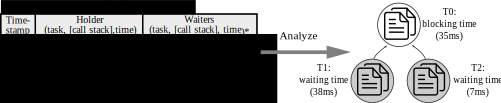
\includegraphics[width=0.80\textwidth]{fig/idleprofiler-idlegraph}
\caption{Example of an idle graph. We create an idle graph by
  analyzing the profiled data. An idle graph represents the relationships
  among critical sections and their waiting and holding tasks.
  The vertex \cc{T0}, \cc{T1}, and \cc{T2} represent call stacks of
  holding and waiting tasks, respectively. The edges show
  holder-waiter relation between the blocker's stack \cc{T0} and the
  waiter's stack \cc{T1} and \cc{T2}.}
\label{f:idleprofiler-idlegraph}
\vspace{-5px}
\end{figure}

